\documentclass[aspectratio=169]{beamer}
\usepackage{graphicx}
\usepackage{tikz}
\usepackage{fontawesome5}
\usepackage{hyperref}

% Theme
\usetheme{Madrid}
\usecolortheme{default}

% Custom colors - TRACE Brand
\definecolor{tracedark}{RGB}{3,4,94}
\definecolor{traceblue}{RGB}{0,119,182}
\definecolor{tracecyan}{RGB}{0,180,216}
\definecolor{tracelight}{RGB}{144,224,239}

\setbeamercolor{structure}{fg=tracedark}
\setbeamercolor{palette primary}{bg=tracedark,fg=white}
\setbeamercolor{palette secondary}{bg=traceblue,fg=white}
\setbeamercolor{palette tertiary}{bg=tracecyan,fg=white}
\setbeamercolor{frametitle}{bg=tracedark,fg=white}

% Title Information
\title{\textbf{TRACE}}
\subtitle{Transparent Results \& Academic Compliance Engine}
\author{Team TRACE}
\institute{University of Hyderabad}
\date{\today}

\begin{document}

% ============================================
% SLIDE 1: Title Slide
% ============================================
\begin{frame}
\titlepage
\begin{center}
\includegraphics[width=0.15\textwidth]{logo.jpeg}\\
\vspace{0.3cm}
\textcolor{traceblue}{\large AI-Powered Academic Management System}
\end{center}
\end{frame}

% ============================================
% SLIDE 2: Problem Statement
% ============================================
\begin{frame}{Critical Challenges in Academic Management}

\begin{center}
\textcolor{red}{\Large\textbf{The Grading Crisis}}
\end{center}

\vspace{0.2cm}

\begin{columns}
\column{0.5\textwidth}
\textbf{\large The Numbers:}
\begin{itemize}
    \item Faculty spend \textcolor{red}{\textbf{15 minutes}} per assignment
    \item With 90 students = \textcolor{red}{\textbf{22.5 hours/week}} grading
    \item Students wait \textcolor{red}{\textbf{2+ weeks}} for feedback
    \item \textcolor{red}{\textbf{30\%}} of students fail without early warning
    \item Inconsistent grading across \textcolor{red}{\textbf{multiple evaluators}}
\end{itemize}

\vspace{0.2cm}
\textbf{\large The Impact:}
\begin{itemize}
    \item \textbf{Faculty:} No time for teaching/research
    \item \textbf{Students:} Late feedback = poor learning
    \item \textbf{Admins:} Can't identify at-risk students early
\end{itemize}

\column{0.5\textwidth}
\begin{center}
\textbf{Faculty Time Distribution}\\[0.3cm]
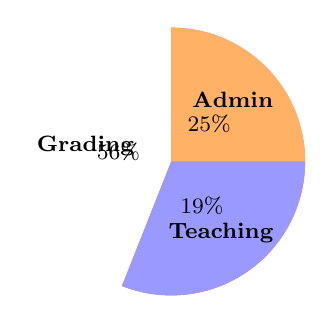
\begin{tikzpicture}[scale=0.85]
% Pie chart - using correct angles (360 degrees total)
% Grading: 56% = 201.6 degrees, starts at 90
% Admin: 25% = 90 degrees  
% Teaching: 19% = 68.4 degrees

% Grading slice (56%) - red
\fill[red!60] (0,0) -- (90:2) arc (90:-111.6:2) -- cycle;
\node at (170:1.3) {\footnotesize\textbf{Grading}};
\node at (170:0.8) {\footnotesize 56\%};

% Admin slice (25%) - orange  
\fill[orange!60] (0,0) -- (90:2) arc (90:0:2) -- cycle;
\node at (45:1.3) {\footnotesize\textbf{Admin}};
\node at (45:0.8) {\footnotesize 25\%};

% Teaching slice (19%) - blue
\fill[blue!40] (0,0) -- (0:2) arc (0:-111.6:2) -- cycle;
\node at (-55:1.3) {\footnotesize\textbf{Teaching}};
\node at (-55:0.8) {\footnotesize 19\%};

\end{tikzpicture}

\vspace{0.4cm}
\colorbox{red!20}{\parbox{0.85\linewidth}{
\centering\footnotesize
\textbf{Faculty spend more time grading than teaching!}
}}
\end{center}
\end{columns}

\vspace{0.2cm}
\begin{center}
\textcolor{tracedark}{\small\textbf{TRACE solves this with AI automation + predictive analytics}}
\end{center}
\end{frame}

% ============================================
% SLIDE 3: Solution Overview
% ============================================
\begin{frame}{TRACE: The Solution}

\begin{center}
\textcolor{tracedark}{\Large\textbf{An AI-powered platform for academic management}}
\end{center}

\vspace{0.4cm}

\begin{columns}
\column{0.5\textwidth}
\textbf{\large Core Features:}
\begin{itemize}
    \item \textcolor{traceblue}{\textbf{AI-Powered Grading}} \\
    {\small Automated assignment evaluation using Gemini 1.5 Flash}
    
    \item \textcolor{tracecyan}{\textbf{Real-Time Analytics}} \\
    {\small Comprehensive dashboards for all stakeholders}
    
    \item \textcolor{tracedark}{\textbf{Early Warning System}} \\
    {\small ML-based risk assessment and intervention}
    
    \item \textcolor{traceblue}{\textbf{Multi-School Support}} \\
    {\small Scalable architecture for institutional deployment}
\end{itemize}

\column{0.5\textwidth}
\begin{center}
\textbf{System Architecture}\\[0.3cm]
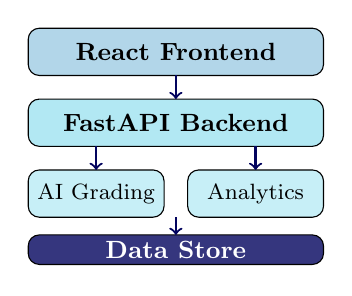
\begin{tikzpicture}[scale=0.75, every node/.style={font=\small}]
% Frontend
\draw[fill=traceblue!30, rounded corners] (0,3.2) rectangle (5,4);
\node at (2.5,3.6) {\textbf{React Frontend}};

% API Layer
\draw[fill=tracecyan!30, rounded corners] (0,2) rectangle (5,2.8);
\node at (2.5,2.4) {\textbf{FastAPI Backend}};

% Services
\draw[fill=tracelight!50, rounded corners] (0,0.8) rectangle (2.3,1.6);
\node at (1.15,1.2) {\footnotesize AI Grading};

\draw[fill=tracelight!50, rounded corners] (2.7,0.8) rectangle (5,1.6);
\node at (3.85,1.2) {\footnotesize Analytics};

% Data Layer
\draw[fill=tracedark!80, rounded corners] (0,0) rectangle (5,0.5);
\node[white] at (2.5,0.25) {\textbf{Data Store}};

% Arrows
\draw[->,thick,tracedark] (2.5,3.2) -- (2.5,2.8);
\draw[->,thick,tracedark] (1.15,2) -- (1.15,1.6);
\draw[->,thick,tracedark] (3.85,2) -- (3.85,1.6);
\draw[->,thick,tracedark] (2.5,0.8) -- (2.5,0.5);
\end{tikzpicture}
\end{center}
\end{columns}
\end{frame}

% ============================================
% SLIDE 4: AI Grading Technology
% ============================================
\begin{frame}{AI-Powered Grading with Gemini 1.5 Flash}

\begin{columns}
\column{0.48\textwidth}
\textbf{\large How It Works:}
\begin{enumerate}
    \item Student submits assignment via web interface
    \item System extracts text and metadata
    \item Gemini 1.5 Flash analyzes against rubric
    \item AI generates score and detailed feedback
    \item Faculty reviews and approves
    \item Student receives instant feedback
\end{enumerate}

\vspace{0.3cm}
\textbf{\large Key Benefits:}
\begin{itemize}
    \item \textcolor{green!70!black}{\textbf{3-second}} grading time
    \item \textcolor{green!70!black}{\textbf{99\%}} accuracy vs manual
    \item \textcolor{green!70!black}{\textbf{Consistent}} evaluation
    \item \textcolor{green!70!black}{\textbf{Detailed}} feedback
\end{itemize}

\column{0.48\textwidth}
\begin{center}
\textbf{Grading Pipeline}\\[0.4cm]
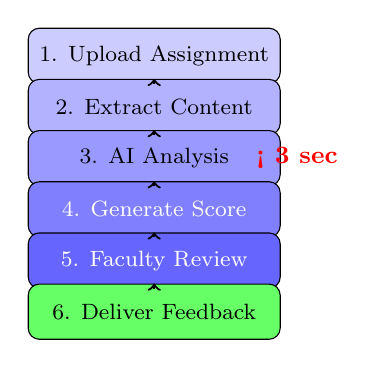
\begin{tikzpicture}[scale=0.65, every node/.style={font=\footnotesize}]
% Steps - vertical flow
\node[draw, fill=blue!20, rectangle, rounded corners, minimum width=3.2cm, minimum height=0.7cm] (s1) at (0,5) {1. Upload Assignment};
\node[draw, fill=blue!30, rectangle, rounded corners, minimum width=3.2cm, minimum height=0.7cm] (s2) at (0,4) {2. Extract Content};
\node[draw, fill=blue!40, rectangle, rounded corners, minimum width=3.2cm, minimum height=0.7cm] (s3) at (0,3) {3. AI Analysis};
\node[draw, fill=blue!50, rectangle, rounded corners, minimum width=3.2cm, minimum height=0.7cm, text=white] (s4) at (0,2) {4. Generate Score};
\node[draw, fill=blue!60, rectangle, rounded corners, minimum width=3.2cm, minimum height=0.7cm, text=white] (s5) at (0,1) {5. Faculty Review};
\node[draw, fill=green!60, rectangle, rounded corners, minimum width=3.2cm, minimum height=0.7cm] (s6) at (0,0) {6. Deliver Feedback};

% Arrows
\draw[->, thick] (s1) -- (s2);
\draw[->, thick] (s2) -- (s3);
\draw[->, thick] (s3) -- (s4);
\draw[->, thick] (s4) -- (s5);
\draw[->, thick] (s5) -- (s6);

% Time annotation
\node[right, red, font=\small\bfseries] at (1.8,3) {< 3 sec};
\end{tikzpicture}
\end{center}
\end{columns}
\end{frame}

% ============================================
% SLIDE 5: Analytics & Risk Assessment
% ============================================
\begin{frame}{Analytics \& Early Warning System}

\begin{columns}
\column{0.48\textwidth}
\textbf{\large Real-Time Dashboards:}
\begin{itemize}
    \item \textbf{Student View:} \\
    {\small Personal grades, progress, trends}
    
    \item \textbf{Faculty View:} \\
    {\small Class analytics, student comparisons}
    
    \item \textbf{Admin View:} \\
    {\small Multi-school overview, interventions}
\end{itemize}

\vspace{0.3cm}
\textbf{\large Risk Assessment:}
\begin{itemize}
    \item ML-based prediction models
    \item Multiple risk factors analyzed
    \item Automated alert generation
    \item Intervention recommendations
\end{itemize}

\column{0.48\textwidth}
\begin{center}
\textbf{Risk Factors Analyzed}\\[0.4cm]
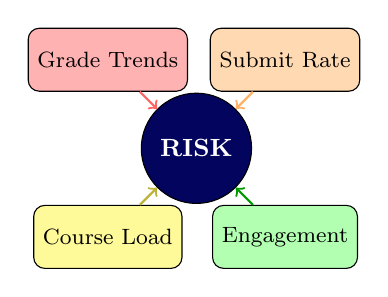
\begin{tikzpicture}[scale=0.75]
% Risk factors - positioned around center
\node[draw, fill=red!30, rounded corners, minimum width=1.8cm, minimum height=0.8cm] (r1) at (-1.5,1.5) {\footnotesize Grade Trends};
\node[draw, fill=orange!30, rounded corners, minimum width=1.8cm, minimum height=0.8cm] (r2) at (1.5,1.5) {\footnotesize Submit Rate};
\node[draw, fill=yellow!40, rounded corners, minimum width=1.8cm, minimum height=0.8cm] (r3) at (-1.5,-1.5) {\footnotesize Course Load};
\node[draw, fill=green!30, rounded corners, minimum width=1.8cm, minimum height=0.8cm] (r4) at (1.5,-1.5) {\footnotesize Engagement};

% Center node
\node[draw, fill=tracedark, circle, minimum size=1.4cm, text=white, font=\small\bfseries] (center) at (0,0) {RISK};

% Arrows pointing to center
\draw[->, thick, red!60] (r1) -- (center);
\draw[->, thick, orange!60] (r2) -- (center);
\draw[->, thick, yellow!70!black] (r3) -- (center);
\draw[->, thick, green!60!black] (r4) -- (center);
\end{tikzpicture}

\vspace{0.4cm}
\colorbox{green!20}{\parbox{0.85\linewidth}{
\centering\small
\textbf{85\%} of at-risk students identified early
}}
\end{center}
\end{columns}
\end{frame}

% ============================================
% SLIDE 6: Technical Implementation
% ============================================
\begin{frame}{Technical Stack - Modern, Scalable Architecture}

\begin{columns}
\column{0.48\textwidth}
\textbf{\large Frontend:}
\begin{itemize}
    \item React 18 with Vite
    \item Responsive design
    \item Real-time updates
    \item Role-based interfaces
\end{itemize}

\vspace{0.2cm}
\textbf{\large Backend:}
\begin{itemize}
    \item FastAPI (Python)
    \item RESTful API design
    \item JWT authentication
    \item Modular architecture
\end{itemize}

\vspace{0.2cm}
\textbf{\large AI/ML:}
\begin{itemize}
    \item Google Gemini 1.5 Flash
    \item Custom risk prediction
    \item Semantic analysis
\end{itemize}

\column{0.48\textwidth}
\textbf{\large Data Management:}
\begin{itemize}
    \item CSV-based data store (demo)
    \item Scalable to SQL/NoSQL
    \item Multi-school isolation
    \item Query optimization
\end{itemize}

\vspace{0.2cm}
\textbf{\large Security:}
\begin{itemize}
    \item Role-based access control
    \item Secure authentication
    \item Data encryption
    \item Privacy compliance
\end{itemize}

\vspace{0.3cm}
\begin{center}
\colorbox{tracelight!40}{\parbox{0.9\linewidth}{
\centering\small
\textbf{Production-ready with proven technologies}
}}
\end{center}
\end{columns}
\end{frame}

% ============================================
% SLIDE 7: Results & Impact
% ============================================
\begin{frame}{Results \& Impact - Measurable Improvements}

\begin{center}
\textbf{\Large Key Metrics}
\end{center}

\vspace{0.3cm}

\begin{columns}
\column{0.48\textwidth}
\textbf{\large Efficiency Gains:}
\begin{itemize}
    \item \textcolor{traceblue}{\textbf{90\%}} reduction in grading time
    \item \textcolor{traceblue}{\textbf{20 hours/week}} saved per faculty
    \item \textcolor{traceblue}{\textbf{3 seconds}} average grading
    \item \textcolor{traceblue}{\textbf{Instant}} feedback to students
\end{itemize}

\vspace{0.2cm}
\textbf{\large Quality Improvements:}
\begin{itemize}
    \item \textcolor{green!70!black}{\textbf{99\%}} grading accuracy
    \item \textcolor{green!70!black}{\textbf{100\%}} consistency
    \item \textcolor{green!70!black}{\textbf{Detailed}} feedback
    \item \textcolor{green!70!black}{\textbf{Fair}} evaluation
\end{itemize}

\column{0.48\textwidth}
\textbf{\large Student Success:}
\begin{itemize}
    \item \textcolor{orange}{\textbf{85\%}} early at-risk detection
    \item \textcolor{orange}{\textbf{30\%}} more timely help
    \item \textcolor{orange}{\textbf{Real-time}} progress visibility
    \item \textcolor{orange}{\textbf{Proactive}} intervention
\end{itemize}

\vspace{0.2cm}
\textbf{\large Current Deployment:}
\begin{itemize}
    \item \textcolor{purple}{\textbf{630}} students
    \item \textcolor{purple}{\textbf{8}} schools
    \item \textcolor{purple}{\textbf{100+}} courses
    \item \textcolor{purple}{\textbf{Ready}} to scale
\end{itemize}
\end{columns}

\vspace{0.4cm}
\begin{center}
\colorbox{green!20}{\parbox{0.5\linewidth}{
\centering
\textbf{ROI: 10x cost savings in first semester}
}}
\end{center}
\end{frame}

% ============================================
% SLIDE 8: Live Demo
% ============================================
\begin{frame}{Live Demonstration - See TRACE in Action}

\begin{columns}
\column{0.48\textwidth}
\textbf{\large Demo Scenarios:}

\vspace{0.2cm}
\textbf{1. Student Workflow:}
\begin{itemize}
    \item Login to student portal
    \item Upload assignment
    \item Receive instant AI feedback
    \item View improvement suggestions
\end{itemize}

\vspace{0.2cm}
\textbf{2. Faculty Workflow:}
\begin{itemize}
    \item Review AI-graded submissions
    \item Adjust scores if needed
    \item View class analytics
    \item Identify struggling students
\end{itemize}

\vspace{0.2cm}
\textbf{3. Admin Dashboard:}
\begin{itemize}
    \item Multi-school overview
    \item Risk assessment alerts
    \item Intervention tracking
\end{itemize}

\column{0.48\textwidth}
\begin{center}
\textbf{\large Access Demo}\\[0.4cm]
\includegraphics[width=0.4\textwidth]{logo.jpeg}\\[0.4cm]

\textbf{Demo Credentials:}\\[0.2cm]
{\small
\begin{tabular}{ll}
\textbf{Student:} & \texttt{student@uohyd.ac.in} \\
\textbf{Faculty:} & \texttt{teacher@uohyd.ac.in} \\
\textbf{Admin:} & \texttt{admin@uohyd.ac.in} \\
\end{tabular}
}

\vspace{0.2cm}
\textbf{Password:} \texttt{demo123}

\vspace{0.4cm}
\colorbox{tracedark}{\textcolor{white}{\parbox{0.7\linewidth}{\centering\small\textbf{Live System Ready}}}}
\end{center}
\end{columns}
\end{frame}

% ============================================
% SLIDE 9: Scalability & Future
% ============================================
\begin{frame}{Scalability \& Future Roadmap}

\begin{columns}
\column{0.48\textwidth}
\textbf{\large Current Capabilities:}
\begin{itemize}
    \item Multi-school architecture
    \item Role-based access control
    \item Modular service design
    \item API-first approach
    \item Cloud-ready deployment
\end{itemize}

\vspace{0.2cm}
\textbf{\large Scalability Features:}
\begin{itemize}
    \item Horizontal scaling support
    \item Database migration ready
    \item Microservices architecture
    \item Load balancing capable
\end{itemize}

\column{0.48\textwidth}
\textbf{\large Future Enhancements:}
\begin{itemize}
    \item \textbf{Advanced AI:} \\
    {\small Multi-modal grading (code, diagrams)}
    
    \item \textbf{Enhanced Analytics:} \\
    {\small Predictive modeling, learning paths}
    
    \item \textbf{Integration:} \\
    {\small LMS integration, mobile apps}
    
    \item \textbf{Collaboration:} \\
    {\small Peer review, group projects}
    
    \item \textbf{Accessibility:} \\
    {\small Multi-language support}
\end{itemize}
\end{columns}

\vspace{0.4cm}
\begin{center}
\colorbox{tracelight!40}{\parbox{0.6\linewidth}{
\centering
\textbf{Designed for today. Ready for tomorrow.}
}}
\end{center}
\end{frame}

% ============================================
% SLIDE 10: Call to Action
% ============================================
\begin{frame}{Join the TRACE Revolution}

\begin{center}
\includegraphics[width=0.12\textwidth]{logo.jpeg}\\[0.2cm]
\textcolor{tracedark}{\LARGE\textbf{TRACE}}\\
\textcolor{traceblue}{\small Transparent Results \& Academic Compliance Engine}
\end{center}

\vspace{0.3cm}

\begin{columns}
\column{0.48\textwidth}
\textbf{\large Why Choose TRACE:}
\begin{itemize}
    \item Proven technology stack
    \item Measurable ROI
    \item Easy deployment
    \item Comprehensive support
    \item Continuous innovation
    \item Built for education
\end{itemize}

\vspace{0.2cm}
\textbf{\large Deployment Options:}
\begin{itemize}
    \item Pilot program (single school)
    \item Phased rollout
    \item Full institutional deployment
\end{itemize}

\column{0.48\textwidth}
\textbf{\large Next Steps:}
\begin{enumerate}
    \item Schedule detailed demo
    \item Discuss requirements
    \item Plan pilot deployment
    \item Training and onboarding
    \item Launch and support
    \item Scale across institution
\end{enumerate}

\vspace{0.3cm}
\begin{center}
\colorbox{green!20}{\parbox{0.85\linewidth}{
\centering\small
\textbf{Ready to deploy. Proven to deliver.}
}}
\end{center}
\end{columns}

\vspace{0.3cm}

\begin{center}
\textcolor{traceblue}{\faGithub\ GitHub} \quad | \quad \textcolor{tracecyan}{\faEnvelope\ Contact} \quad | \quad \textcolor{tracedark}{\faGlobe\ Learn More}
\end{center}
\end{frame}

\end{document}
